\documentclass[12pt]{report}
\usepackage[pdftex]{graphicx}
\usepackage[margin=1.2in]{geometry}
\usepackage{listings}
\usepackage{xcolor}

\definecolor{codegreen}{rgb}{0,0.6,0}
\definecolor{codegray}{rgb}{0.5,0.5,0.5}
\definecolor{codepurple}{rgb}{0.58,0,0.82}
\definecolor{backcolour}{rgb}{0.95,0.95,0.92}

\lstdefinestyle{mystyle}{
    backgroundcolor=\color{backcolour},   
    commentstyle=\color{codegreen},
    keywordstyle=\color{magenta},
    numberstyle=\tiny\color{codegray},
    stringstyle=\color{codepurple},
    basicstyle=\ttfamily\footnotesize,
    breakatwhitespace=false,         
    breaklines=true,                 
    captionpos=b,                    
    keepspaces=true,                 
    % numbers=right,                    
    numbersep=5pt,                  
    showspaces=false,                
    showstringspaces=false,
    showtabs=false,                  
    tabsize=2
}

\lstset{style=mystyle}



% \usepackage{graphicx} %package to manage images
\graphicspath{{./images/}}
\newcommand*\lstinputpath[1]{\lstset{inputpath=#1}}
\lstinputpath{codes}

\begin{document}

\tableofcontents

\chapter{Introduction to Machine Learning}
Machine Learning is undeniably one of the most influential and powerful technologies in today’s world. It is a tool for turning information into knowledge. In the past 50 years, there has been an explosion of data. This mass of data is useless unless we analyze it and find the patterns hidden within. Machine learning techniques are used to automatically find the valuable underlying patterns within complex data that we would otherwise struggle to discover. The hidden patterns and knowledge about a problem can be used to predict future events and perform all kinds of complex decision making.\\\\
There are multiple forms of Machine Learning; supervised, unsupervised , semi-supervised and reinforcement learning. Each form of Machine Learning has differing approaches, but they all follow the same underlying process and theory. I'll cover supervised and unsupervised learning for my report.


\section{Supervised and Unsupervised Learning}
  The most basic thing to remember is that we already know what our correct output should look like in Supervised Learning.
  But, we have little or no idea about what our results should look like.

  \textbf{Supervised Learning:}
  \begin{itemize}
    \item Classification: Spam/Not-spam. 
    \item Regression: Predicting age.
  \end{itemize}

  \textbf{Unsupervised Learning:}
  \begin{itemize}
    \item Clustering: Grouping based on different variables.
    \item Non Clustering: Finding structure in a chaotic environment.
  \end{itemize}


\chapter{Linear Regression}
\section{Linear Regression with one variable}
  Regression being a part of Supervised Learning is used for estimatng data (Real-valued output).  

  \subsection{Cost Function}
    This function measures the performance of a Machine Learning model for given data.

    \textbf{Hypothesis}: $ h_ \theta(x) = \theta_0 + \theta_1x $

    \textbf{Parameters:} $ \theta_0, \theta_1 $

    \textbf{Cost Function:} 
    \begin{equation} \label {eq:1}
      J( \theta_0, \theta_1 ) = 1/2m \sum_{i=1}^{m} (h_\theta(x^{(i)})-y^{(i)})^2 
    \end{equation} 

    \textbf{Goal:} Minimize cost function with $ \theta_0, \theta_1 $ as parameters.

  \subsection{Gradient Descent}

    \textbf{Basic idea:}
    \begin{itemize}
    \item Start with some $ \theta_0, \theta_1 $
    \item Keep changing $ \theta_0, \theta_1 $ to reduce $ J(\theta_0, \theta_1) $ until we end up at minima.
    \end{itemize} 

    \textbf{Algorithm:}
     repeat until convergence:
    \begin{equation} \label {eq:2}
      \theta_j := \theta_j - \alpha \frac{\partial {J(\theta_0, \theta_1)}}{\partial \theta_j}
    \end{equation} 

    (for  $j = 0, 1 $  ,here).  

    \textbf{Intution:} 
    If $\alpha$ is too small, descent can be slow and if too large, descent may fail to converge or even diverge.
    Gradient descent can converge to a local minimum, even with fixed learning rate $\alpha$. As we approach local mimimum, gradient descent will automatically take smaller steps. So, no need to decrease $\alpha$ over time. 

  \subsection{Gradient Descent for linear regression}
    Combining gradient descent algorithm with linear regression model, we get:

    \begin{equation} \label {eq:3}
      j = 0 : \frac{\partial {J(\theta_0, \theta_1)}}{\partial \theta_0} = 1/2 \sum_{i=1}^{m} (h_\theta(x^{(i)})-y^{(i)}) 
    \end{equation}

    \begin{equation} \label {eq:4}
      j = 1 : \frac{\partial {J(\theta_0, \theta_1)}}{\partial \theta_1} = 1/2 \sum_{i=1}^{m} (h_\theta(x^{(i)})-y^{(i)}).x^{(i)}
    \end{equation}

    Now, we can repeat \ref{eq:3} and \ref{eq:4} until convergence to obtain the minima.

    "Batch" gradient descent: Each step of gradient descent uses all the training examples.
    For eq. "m" batches in equation \ref{eq:1}.

\section{Multivariate Linear Regression}
  Linear regression involving more than one variable. For eq., Predicting price of a house based on parameters "Plot Area", "No. of Floors", "Connectivity with markets", etc.

  \subsection{Multiple Features}
    The multivariable form of the hypothesis is as follows:
    \begin{equation} \label {eq:5}
      h_\theta(x) = \theta_0 + \theta_1x_1 + \theta_2x_2 + \theta_ 3x_3 + ... + \theta_{n}x_n.  
    \end{equation}
    This hypothesis funtion can be concisely represented as:
    \begin{equation}
      h_\theta(x) = \theta^{T}x
    \end{equation}
    where, $ \theta^T $ is a 1xn matrix consisting of $ \theta_0, \theta_1, \theta_2 ... \theta_n $.


  \subsection{Gradient Descent for Multiple Variables}
    Gradient descent formula for Multiple variable will be similar to that of single variable.

    \begin{equation} \label {eq: GD for multiple}
      \theta_j =  \theta_j - \alpha \frac{1}{m} \sum_{i=1}^{m} (h_\theta(x^{(i)})-y^{(i)}).x_j^{(i)}
    \end{equation}

    Repeating this equation until convergence will give the minima. \footnote[1]{$x_0 = 1$ in equation \ref{eq: GD for multiple}}

  \subsubsection{Feature Scaling}
    Feature Scaling is used to reduce the number of iterations in Gradient Descent. Basic idea of feature scaling is to bring all the features on the same scale. (in general we try to approximate every feature in the range $ -1 < x_i < 1 $)
    \\ \\ Reducing the number of iteration doesn't mean making computation of each step easier. And also it does not effect comtational efficiency of Normal Equation.

  \subsubsection{Mean Normalisation}
    Mean Normalisation makes features to have approximately zero mean.

  \subsubsection{Learning Rate}
    If $\alpha$ is too small: slow convergence.

    if $\alpha$ is too large: $J(\theta)$ may not decrease on every iteration, or may not converge.

  \subsubsection{Polynomial Regression}
    Selecting proper polynomial for fitting data is very important.

    \begin{figure}[h]
      \centering
      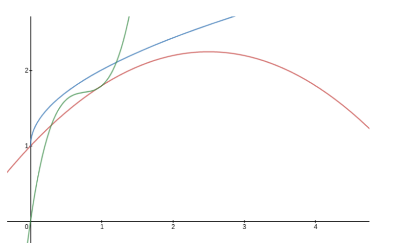
\includegraphics[width=8cm, height=5cm]{polyreg.png}
    \end{figure}

    \textbf{Red:} Quadratic

    \textbf {Blue:} Square root funtion $ \theta_0+\theta_1x+\theta_2\sqrt{x} $

    \textbf {Green:} Cubic function

\section{Normal equation}
  Normal Equation is a method to solve for $\theta_T$ analytically, by creating a $m\times(n+1)$ matrix $X$ and another $m\times1$ matrix $Y$.\footnote[2]{Every element of first column of matrix $X$ is 1 and other are the feature's coefficient}

  Mathematically $\theta$ is given as:
  \begin{equation} \label {eq: theta}
    \theta = (X^TX)^{-1}X^ty
  \end{equation}

  \begin{tabular}{ |c|c|}
    \hline
    \textbf{Gradient Descent} & \textbf{Normal Equation} \\
    \hline
    Need to choose $\alpha$ & No need to choose $\alpha$ \\
    Needs many iteration & Don't need to iterate \\
    Works well with large n & Slow for large n \\
    \hline
  \end{tabular}

  \vspace{5mm}

  \subsubsection{Reasons for non-invertiblity of $X^T X$}
    \begin{itemize}
      \item Redundant features (linear dependence) \footnote[3]{Eg. Using both $m^2 \  \& \  (feet)^2$ features}
      \item Too many features (m $<=$ n) 
    \end{itemize}


\chapter{Logistic Regression}
\section{Classification and Representation}

  \subsection{Classification}
    The classification problem is just like the regression problem, except that the values we now want to predict take on only a small number of discrete values. For now, we'll discuss a binary classification problem.

  \subsection{Hypothesis Representation}
    We may use our old regression algorithm by classifying data on the basis of a threshold. But it will have very poor performance.\\ 
    \\We will introduce "Sigmoid Function", also called the "Logistic Function":
    \begin{equation}
      h_\theta(x) = g(\theta^{T}x)
    \end{equation}
    \begin{equation}
      z = \theta^{T}x
    \end{equation}
    \begin{equation}\label{eq:sigmoid}
      g(z) = \frac{1}{1+e^{-z}}
    \end{equation}
    This is how the Sigmoid Function looks like:
    \begin{figure}[h]
      \centering
      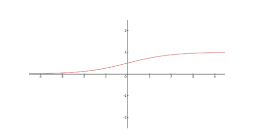
\includegraphics[scale = 0.6]{sigmoid.png}
      \caption{Sigmoid Funtion \ref{eq:sigmoid}}
    \end{figure}

  \subsection{Decesion Boundary}
    The decision boundary is the line that separates the area where y=0 and where y=1.\\
    It is similar to the decision boundary for linear regression, the only difference is the distribution of values (linear and sigmoid)

\section{Logistic Regression Model}

  \subsection{Cost Function}
    Cost funtion for logistic regression looks like:

    \begin{equation}
      J(\theta) = \frac{1}{m}\sum_{i=1}^{m}Cost(h_\theta(x^{(i)}), y^{(i)})
    \end{equation}
    \\ \\
    $ Cost(h_\theta(x),y) = -\log{(h_\theta{(x)})} $ \hfill if $y = 1$
    \\ \\
    $Cost(h_\theta(x),y) = -\log{(1-h_\theta{(x)})}$  \hfill if $y = 0$

    \begin{figure}[h]
      \centering
      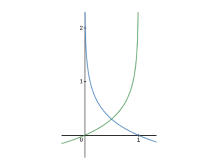
\includegraphics[scale = 0.6]{costlog.png}
      \caption{Cost Funtion}
    \end{figure}

    \subsubsection{Siplified Cost Funtion}
    This cost funtion can be compressed into a single funtion:
    \begin{equation}
      Cost(h_\theta(x),y) = -y\log{(h_\theta{(x)})} -(1-y)\log{(1-h_\theta{(x)})}
    \end{equation}
    A vectorised implementation is: \\ \\
    $h = g(X\theta)$\\
    $J(\theta) = \frac{1}{m}.(-y^T\log{h}-(1-y)^T\log{1-h})$
    \\ \\
    Vectorised implementation for Gradient Descent: \\ \\
    $\theta := \theta - \frac{\alpha}{m}X^T(g(X\theta)-y)$

\section{Multiclass Classification}
  \subsection{One-vs-all}
    This approach is when data has more than two categories.We divide our problem into n\footnote[1]{n = no of categories in dataset} binary classification problems, in each one, we predict the probability considering one of the category to be $+$ve and all other to be $-$ve. Repeating this for all other categories will finally give us all the decesion boundaries.
    \begin{figure}[h]
      \centering
      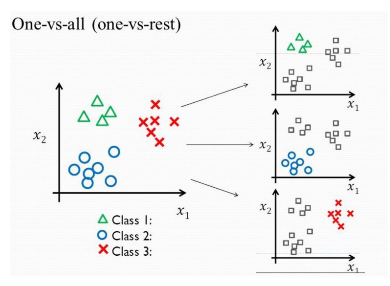
\includegraphics[scale = 0.5]{oneall.png}
      \caption{One vs all classifiaction method}
    \end{figure}   

\section{The Problem of Overfitting}
  Consider the problem of predicting y from x $\in$ R. The leftmost figure below shows the result of fitting a $y = \theta_0+\theta_1x$ to a dataset. We see that the data doesn’t really lie on straight line, and so the fit is not very good.\\ 
  \begin{figure}[h]
    \centering
    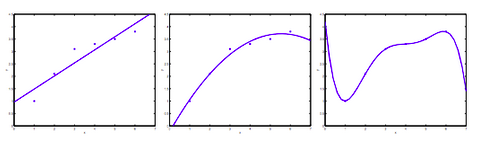
\includegraphics[scale=0.5]{overfitting.png}
  \end{figure}
  \\
  Instead, if we had added an extra feature $x^2$ , and fit $ t = \theta_0 + \theta_1x + \theta_2x^2$ , then we obtain a slightly better fit to the data (See middle figure). Naively, it might seem that the more features we add, the better. However, there is also a danger in adding too many features: The rightmost figure is the result of fitting a $5^{th}$ order polynomial $y = \sum_{j=0} ^5 \theta_j x^j$. We see that even though the fitted curve passes through the data perfectly, we would not expect this to be a very good predictor of, say, housing prices (y) for different living areas (x). Without formally defining what these terms mean, we’ll say the figure on the left shows an instance of \textbf{underfitting}—in which the data clearly shows structure not captured by the model—and the figure on the right is an example of \textbf{overfitting}.

    \subsubsection{How to address this issue?}
      \begin{enumerate}
        \item Reduce the number of features:
        \begin{itemize}
          \item Manually select which features to keep.
          \item Use a model selection algorithm.\footnote[2]{we'll cover it later}
        \end{itemize}
        \item Regularisation:
        \begin{itemize}
          \item Keep all the features, but reduce the magnitude of parameters $\theta_j$.
          \item Regularization works well when we have a lot of slightly useful features.
        \end{itemize}
      \end{enumerate}

  \subsection{Regularized Cost Function}
    To solve this problem of overfitting, we can eleminate the influence of $\theta_3x^3$ and $\theta_4x^4$. Without actually getting rid of these features or changing the form of our hypothesis, we can instead modify our cost function:
    \begin{equation}
      J_\theta = min\ of\ \left[ \frac{1}{2m} \sum_{i=1}^{m}(h_\theta(x^{(i)}) - y^{(i)})^2 + \lambda\sum_{j=1}^2\theta_j^2 \right]
    \end{equation}
    These extra terms will inflate the cost of extra parameters. \\ \\
    The $\lambda$ is called the \textbf{regularisation parameter}/ It determines how much the costs of out theta parameters are inflated.

  \subsection{Regularized Linear Regression}
    \begin{figure}[h]
      \centering
      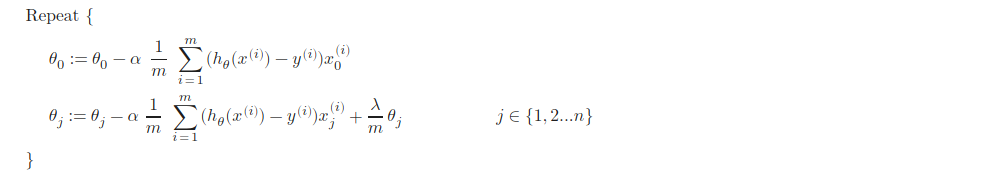
\includegraphics[scale=1]{gradregularize.png}
    \end{figure}


    The term $\frac{\lambda}{m}\theta_{j}$ performs our regularization. With some manipulation, our update rule can also be represented as \\

    $ \theta_j := \theta_j(1 - \alpha\frac{\lambda}{m}) - \alpha\frac{1}{m}\sum_{i=1}^m(h_\theta(x^{(i)}) - y^{(i)})x_j^{(i)} $\\

    The first term in the above equation, $\alpha\frac{\lambda}{m}$ will always be less than 1. Intuitively you can see it as reducing the value of $j\theta_j$ by some amount on every update.

    \subsubsection{Normal Eequation}
      This will be the non-iterative approach for regularisation.\\\\
      To add in regularization, we'll just add another term:
      \begin{equation}
        \theta = X^T X + \lambda . L^{-1} X^T y
      \end{equation}
      where, L is $(n+1)\times(n+1)$ matrix with 0 at the top lest, 1`s down the diagonal and all other element '0'.
    % \\ \\
    % \lstinputlisting[language=Octave, caption=Octave Implementation for Logistic Regression Algorithms]{logisticRegression.m}


\chapter{Neural Networks}
  At a very simple level, neurons are basically computational units that take inputs (\textbf{dendrites}) as electrical inputs (called "spikes") that are channeled to outputs (\textbf{axons}). In our model, our dendrites are like the input features $x_1...x_n$, and the output is the result of our hypothesis function. In this model our $x_0$ input node is sometimes called the "bias unit." It is always equal to 1.

  \begin{figure}[h]
    \centering
    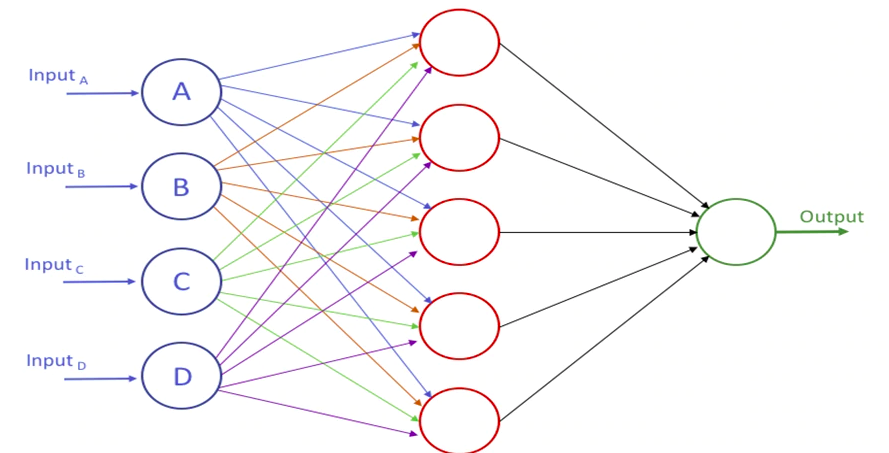
\includegraphics[scale=0.3]{neuralnetwork.png}
  \end{figure}

  Our input nodes (layer 1), also known as the "input layer", go into another node (layer 2), which finally outputs the hypothesis function, known as the "output layer". We can have intermediate layers of nodes between the input and output layers called the "hidden layers."
  \\\\
  These "hidden layer" nodes are called as "activation units". The values for each activation nodes are represented as: \\
  \begin{figure}[h]
    \centering
    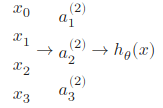
\includegraphics[scale=0.6]{hiddenlayer.png}
  \end{figure}

  \begin{equation}
    a_1^{(2)} = g(\theta_{10}^{(1)}x_0 + \theta_{11}^{(1)}x_1 + \theta_{12}^{(1)}x_2 + \theta_{13}^{(1)}x_3)
  \end{equation}
  \begin{equation}
    a_2^{(2)} = g(\theta_{20}^{(1)}x_0 + \theta_{21}^{(1)}x_1 + \theta_{22}^{(1)}x_2 + \theta_{23}^{(1)}x_3)
  \end{equation}
  \begin{equation}
    a_3^{(2)} = g(\theta_{30}^{(1)}x_0 + \theta_{31}^{(1)}x_1 + \theta_{32}^{(1)}x_2 + \theta_{33}^{(1)}x_3)
  \end{equation}
  \begin{equation}
    h_\theta(x) = a_1^{(3)]} = a_1^{(2)} = g(\theta_{10}^{(2)}x_0 + \theta_{11}^{(2)}x_1 + \theta_{12}^{(2)}x_2 + \theta_{13}^{(2)}x_3)5
  \end{equation}
  \\From these equations, we can conclude that we will get a matrix for each layer to calculate the weight for the second layer.

  \section{Intutions}
    \subsection{OR Function}
      \begin{figure}[h]
        \centering
        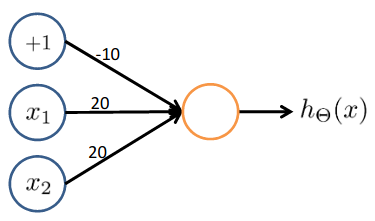
\includegraphics[scale=0.5]{ornet.png}
        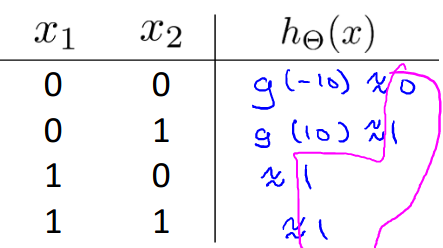
\includegraphics[scale=0.4]{ortable.png}
      \end{figure}

    \subsection{Important Note}
      \begin{figure}[h]
        \centering
        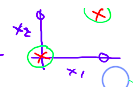
\includegraphics[scale=1]{important-net.png}
      \end{figure}

      For any prediction which involves a straight line as decision boundary, we can represent it with a neural network without any hidden layer but otherwise, we'll have to include few hidden layers. An important point to note is that we can represent almost any distribution with a certain arrangement of Neural Network.

  \section{Multiclass Classification}
    To classify data into multiple classes, we'll have to define out set of resulting classes as y:
    \begin{figure}[h]
      \centering
      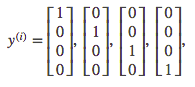
\includegraphics[scale=0.6]{resultnet.png}
    \end{figure}

  \section{Cost Function}
    Let's first define a few variables that we'll need to use:
    
    \begin{itemize}
      \item L = total number of layers in the network
      \item numbers of units (non counting bias unit) in layer 1
      \item K = numbet of output unit/classes
    \end{itemize}

    The cost function for neural networks will be slightly more complicated as it involves a few other factors of 'K' and 'L' defined earlier.

    \begin{equation}
      J(\theta) = -\frac{1}{m}\sum_{i=1}^{m}\sum_{k=1}^{K}y_k^{(i)}\log((h_\theta(x^{(i)}))_k) + (1-y_k^{(i)})\log(1-(h_\theta(x^{(i)}))_k) + \frac{\lambda}{2m}\sum_{l=1}^{L-1}\sum_{i=1}^{s_l}\sum_{j=1}^{s_{l+1}} (\theta_{j,i}^{(L)})^2
    \end{equation}

    \textbf{Note:}
    \begin{itemize}
      \item the double sum simply adds up the logistic regression costs calculated for each cell in the output layer.
      \item the triple sum simply adds up the squares of all the individual $\theta$s in the entire network.
      \item the I in the triple sum does not refer to training example i.
    \end{itemize}

  \section{Backpropagation Algorithm}
    Given training set ${(x^(1),y^(1))...(x^(m),y^(m))}$
    \begin{itemize}
      \item Set $\Delta^{(l)}_{i,j} := 0$ for all (l,i,j), (hence you end up having a matrix full of zeros)
    \end{itemize}

    For training example t=1 to m:
    \begin{enumerate}
      \item Set $a^{(1)} := x^{(t)}$
      \item Perform forward propagation to compute $a^{(l)}$ for l = 2,3,...,L

      \textbf{Gradient Computation}

      \item Using $y^{(t)}$, compute $\delta^{(L)} = a^{(L)} - y^{(L)}$
      \item Compute $\delta^{(l)}$
      \item $\Delta^{(L)} := \Delta^{(L)} + \delta^{(l+1)}(a^{(l)})^T$

      \begin{figure}[h]
        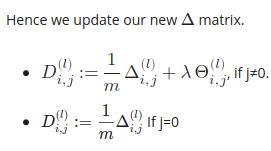
\includegraphics[scale=0.65]{bpupdate.png}
      \end{figure}
    \end{enumerate}

  \section{Gradient Checking}
    Gradient checking will assure that our backpropagation works as intended. We can approximate the derivative of our cost function with:

    \begin{figure}[h]
      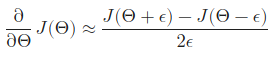
\includegraphics[scale=0.65]{gc.png}
    \end{figure}

    And for multiple features,

    \begin{figure}[h]
      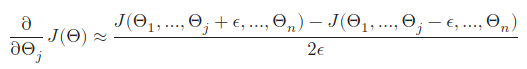
\includegraphics[scale=0.65]{gcmult.png}
    \end{figure}

  \section{Putting it Together}
    First, pick a network architecture; choose the layout of your neural network, including how many hidden units in each layer and how many layers in total you want to have.

    \begin{itemize}
      \item Number of input units = dimension of features $x^{(i)}$
      \item Number of output units = number of classes
      \item Number of hidden units per layer = usually more the better (must balance with the cost of computation as it increases with more hidden units)
      \item Defaults: 1 hidden layer. If you have more than 1 hidden layer, then it is recommended that you have the same number of units in every hidden layer.
    \end{itemize}

    \subsubsection{Training a Neural Network}
      \begin{enumerate}
        \item Randomly initialize the weights\footnote[3]{A good choice for $e_init = \frac{\sqrt{6}}{\sqrt{L_in + L_out}}$}
        \item Implement forward propagation to get $h_\theta(x(i))$ for any $x^{(i)}$
        \item Implement the cost function
        \item Implement backpropagation to compute partial derivatives
        \item Use gradient checking to confirm that your backpropagation works. Then disable gradient checking.
        \item Use gradient descent or a built-in optimization function to minimize the cost function with the weights in theta.
      \end{enumerate}

  % \lstinputlisting[language=octave, caption=Octave implementation for section of Neural Networks]{3.NeuralNetwork.m}

\chapter{Improving Neural Networks}
What to try next for improving our neural networks?
\begin{itemize}
  \item Getting more training examples
  \item Trying smaller sets of features
  \item Trying additional features
  \item Trying polynomial features
  \item Increasing or decreasing $\lambda$
\end{itemize}

\section{Evaulating a Hypothesis}
A hypothesis may have a low error for training examples but still be inaccurate (because of overfitting). Thus, to evaulate a hypothesis, given a dataset of training examples, we can split up the data into two sets: a training set and a test set. Typically, the training set consists of $70\%$ of your data and the test set is the remaining $30\% $.

\begin{figure}[h]
  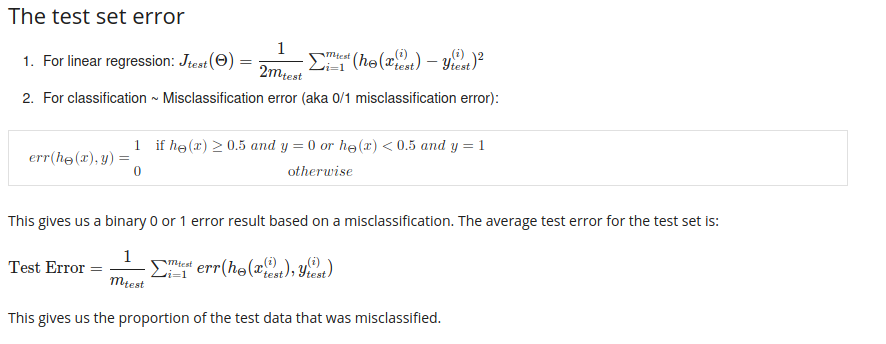
\includegraphics[scale=0.5]{testerror.png}
\end{figure}

\subsection{Model Selection}
  Just because a learning algorithm fits a training set well, that does not mean it is a good hypothesis. It could over fit and as a result your predictions on the test set would be poor.
  \\\\
  Given many models with different polynomial degrees, we can use a systematic approach to identify the 'best' function. In order to choose the model of your hypothesis, you can test each degree of polynomial and look at the error result.
  \\\\
  We usually break down out dataset into three sets:
  \begin{itemize}
    \item Training set: $60\%$
    \item Cross validation set: $20\%$
    \item Test set: $20\%$
  \end{itemize}


  Now to improve our training:
  \begin{enumerate}
    \item Optimize the parameters in $\theta$ using training set.
    \item Find the polynomial degree $d$ with the least error usign the cross validation set.
    \item Estimate the generalization error using the test set with $J_{test}(\Theta^{(d)})$ (d = $\theta$ from polynomial with lower error)
  \end{enumerate}

\section{Bias vs. Variance}
  \textbf{High bias (underfitting)}: both $J_train(\theta)$ and $J_{CV}(\theta)$ will be high and also similar.
  \\\\
  \textbf{High variance (overfitting)}: $J_train(\theta)$ will be low but $J_{CV}(\theta)$.\\

  \begin{figure}[h]
    \centering
    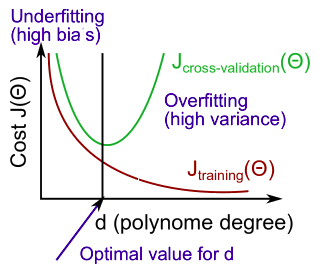
\includegraphics[scale=0.5]{biasVariance.png}
  \end{figure}

  \subsection{Regularization}

    \begin{figure}[h]
      \centering
      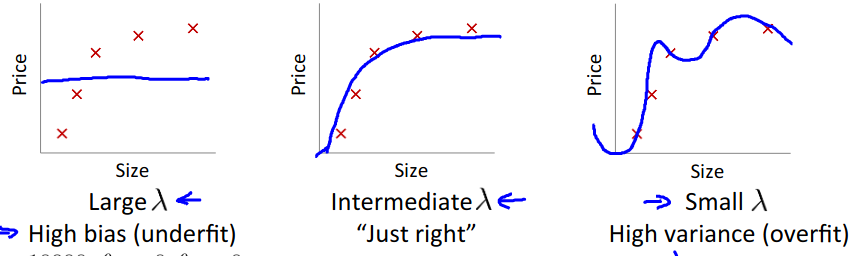
\includegraphics[scale=0.5]{lambda.png}
      \caption{Fitting of data with $\lambda$}
    \end{figure}

    In the figure above, we see that as $\lambda$ increases, our fit becomes more rigid. On the other hand, as $\lambda$ approaches 0, we tend to over overfit the data. So how do we choose our parameter $\lambda$ to get it 'just right' ?

    \begin{enumerate}
      \item Create a list of lambdas.
      \item Iterate through the $\lambda s$ and for each, go throught all the models to learn some $\theta$
      \item Compute the cross validation error.
      \item Select the best combo of $\theta \& \lambda$.
    \end{enumerate}    

  \subsection{Learning Curves}
    \begin{figure}[h]
      \centering
      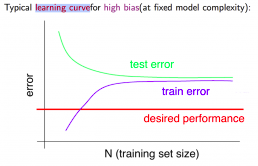
\includegraphics[scale=0.7]{learnbias.png}
      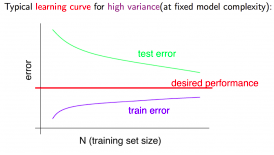
\includegraphics[scale=0.75]{learnvariance.png}
    \end{figure}    
  


\chapter{Unsupervised Learning}
Unsupervised learning is a type of machine learning that looks for previously undetected patterns in a data set with no pre-existing labels and with a minimum of human supervision. In contrast to supervised learning that usually makes use of human-labeled data, unsupervised learning, also known as self-organization allows for modeling of probability densities over inputs. It forms one of the three main categories of machine learning, along with supervised and reinforcement learning. Semi-supervised learning, a related variant, makes use of supervised and unsupervised techniques.

\section{K-Means Clustering Algorithm}
	Kmeans algorithm is an iterative algorithm that tries to partition the dataset into K pre-defined distinct non-overlapping subgroups (clusters) where each data point belongs to only one group. It tries to make the intra-cluster data points as similar as possible while also keeping the clusters as different (far) as possible. It assigns data points to a cluster such that the sum of the squared distance between the data points and the cluster’s centroid (arithmetic mean of all the data points that belong to that cluster) is at the minimum. The less variation we have within clusters, the more homogeneous (similar) the data points are within the same cluster.\\\\

	The way kmeans algorithm works is as follows:
	\begin{enumerate}
		\item Specify number of clusters K.
		\item Initialize centroids by first shuffling the dataset and then randomly selecting K data points for the centroids without replacement.
		\item Keep iterating until there is no change to the centroids. i.e assignment of data points to clusters isn’t changing: 
		\begin{itemize}
			\item Compute the sum of the squared distance between data points and all centroids.
			\item Assign each data point to the closest cluster (centroid).
			\item Compute the centroids for the clusters by taking the average of the all data points that belong to each cluster.
		\end{itemize}
	\end{enumerate}

	\subsection{\textbf{The Elbow Method}: Choosing the number of clusters}
		For the k-means clustering method, the most common approach for choosing the number of clusters is the so-called \textbf{elbow method}. It involves running the algorithm multiple times over a loop, with an increasing number of cluster choice and then plotting a clustering score as a function of the number of clusters.\\

		What is the score or metric which is being plotted for the elbow method? Why is it called the ‘elbow’ method?\\

		A typical plot looks like following,

		\begin{figure}[h]
			\centering
			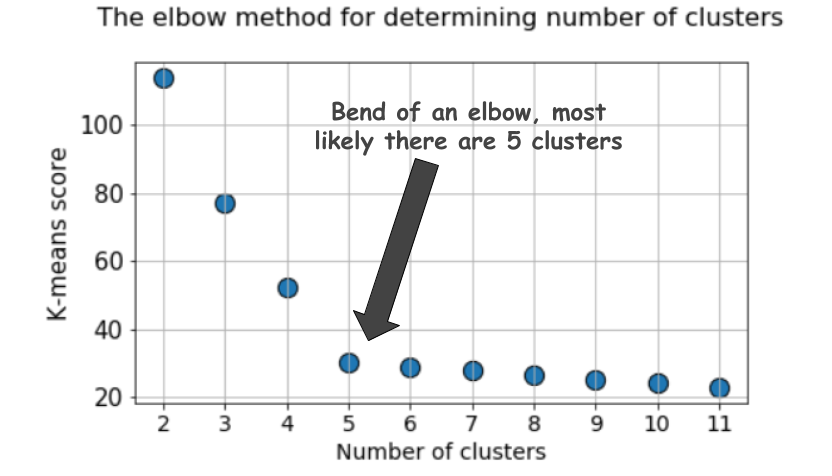
\includegraphics[scale=0.35]{elbow.png}
			\caption{Elbow Method: Score plot}
		\end{figure}

		The score is, in general, a measure of the input data on the k-means objective function i.e. \textbf{some form of intra-cluster distance relative to inner-cluster distance}.

\chapter{Octave/MATLAB Commands}
\subsubsection{Basic Operations}
\begin{lstlisting}[basicstyle=\small]
octave:1> a = pi
a =  3.1416
octave:2> disp(sprintf('6 decimals: %0.6f', a))
6 decimals: 3.141593
octave:3> a
a =  3.1416
octave:4> format long
octave:5> a
a =  3.141592653589793
octave:6> format short
octave:7> a
a =  3.1416
octave:8> v = 1:0.1:2
v =

    1.0000    1.1000    1.2000    1.3000    1.4000    1.5000    1.6000    1.7000    1.8000    1.9000    2.0000

octave:9> v = 1:0.1:2
v =

 Columns 1 through 8:

    1.0000    1.1000    1.2000    1.3000    1.4000    1.5000    1.6000    1.7000

 Columns 9 through 11:

    1.8000    1.9000    2.0000

octave:10> v = 1:6
v =

   1   2   3   4   5   6

octave:11> zeros(1,3)
ans =

   0   0   0

octave:12> rand(1,3)
ans =

   0.43623   0.76554   0.23635

octave:13> randn(1,3)
ans =

   0.5602642  -0.0043628   0.1344922

octave:14> w = -6 + sqrt(10)*(randn(1,10000))

octave:15> hist(w)
\end{lstlisting}

\begin{figure}[h]
  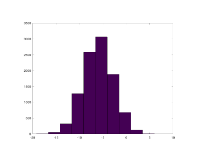
\includegraphics[width=4cm, height=3cm]{hist.png}
\end{figure}

\begin{lstlisting}[basicstyle=\small]
octave:1> w = -6 + sqrt(10)*(rand(1,10000));

octave:2> hist(w,50)
\end{lstlisting}

\begin{figure}[h]
  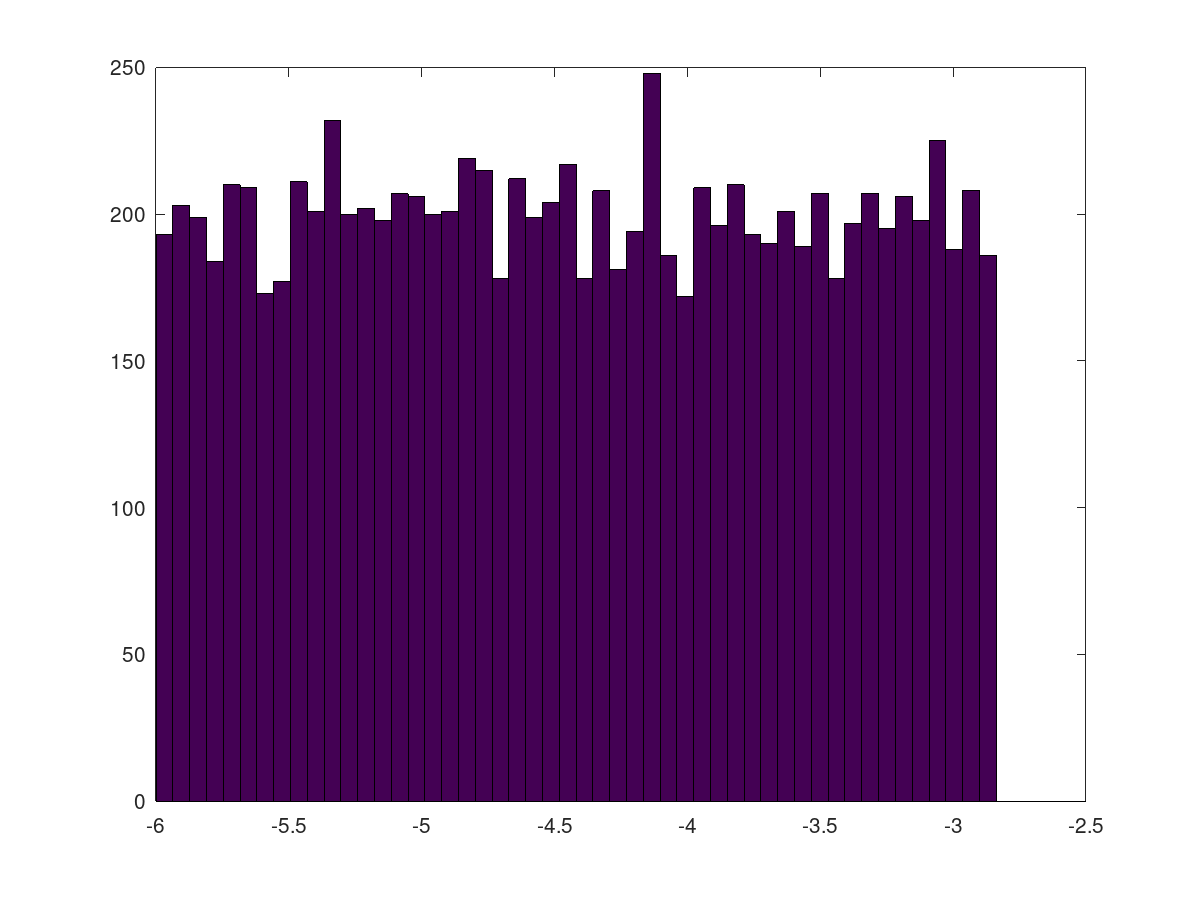
\includegraphics[width=4cm, height=3cm]{hist2.png}
\end{figure}

\subsubsection{Moving Data around}
\begin{lstlisting}[basicstyle=\small]
octave:1> A = [1,2;3,4;4,5]
A =

   1   2
   3   4
   4   5

octave:2> size(A)
ans =

   3   2

octave:3> sz = size(A)
sz =

   3   2

octave:4> size(sz)
ans =

   1   2

octave:5> size(A,1)
ans =  3
octave:6> size(A,2)
ans =  2
octave:7> length(A)
ans =  3
octave:8> length([1,2,3,4,5])
ans =  5
octave:9> 
octave:9> 
octave:9> pwd
ans = /home/sahasra
octave:10> cd /home/sahasra/
octave:11> pwd
ans = /home/sahasra
octave:12> ls
Android          Documents   Music     Public     Videos
AndroidStudioProjects  Downloads   MyPaint   snap
Desktop          examples.desktop  Pictures  Templates
octave:13> who
Variables in the current scope:

A    ans  sz

octave:14> whos
Variables in the current scope:

   Attr Name        Size                     Bytes  Class
   ==== ====        ====                     =====  ===== 
        A           3x2                         48  double
        ans         1x13                        13  char
        sz          1x2                         16  double

Total is 21 elements using 77 bytes

octave:15> clear
octave:16> whos
octave:17> A = [1,2;3,4;5,6]
A =

   1   2
   3   4
   5   6

octave:18> A(3,2)
ans =  6
octave:19> A(2,:)
ans =

   3   4

octave:20> A(:,2)
ans =

   2
   4
   6

octave:21> A([1,3], :)
ans =

   1   2
   5   6

octave:22> A([2,3], :)
ans =

   3   4
   5   6

octave:23> A(:,2) = [10;11;12]
A =

    1   10
    3   11
    5   12

octave:24> A = [A, [5;6;7]]
A =

    1   10    5
    3   11    6
    5   12    7

octave:25> A(:)
ans =

    1
    3
    5
   10
   11
   12
    5
    6
    7

octave:26> A
A =

    1   10    5
    3   11    6
    5   12    7

octave:27> B = [45;46;47]
B =

   45
   46
   47

octave:28> C = [A,B]
C =

    1   10    5   45
    3   11    6   46
    5   12    7   47


\end{lstlisting}


\subsubsection{Computing on Data}
\begin{lstlisting}[basicstyle=\small]
octave:1> A = [1 2;3 4;5 6]
A =

   1   2
   3   4
   5   6

octave:2> B = [11 12; 13 14; 15 16]
B =

   11   12
   13   14
   15   16

octave:3> C = [1  1; 2 2]
C =

   1   1
   2   2

octave:4> A*C
ans =

    5    5
   11   11
   17   17

octave:5> A .* B % A .* B gives element wise operation
ans =

   11   24
   39   56
   75   96

octave:6> 1 ./ A
ans =

   1.00000   0.50000
   0.33333   0.25000
   0.20000   0.16667

octave:7> v = [1;2;3]
v =

   1
   2
   3

octave:8> log(v)
ans =

   0.00000
   0.69315
   1.09861

octave:9> exp(v)
ans =

    2.7183
    7.3891
   20.0855

octave:10> abs([-1; 2; -3])
ans =

   1
   2
   3

octave:11> A
A =

   1   2
   3   4
   5   6

octave:12> A' % A' = A transpose
ans =

   1   3   5
   2   4   6

octave:13> val = max([1;2;3;6;7])
val =  7
octave:14> max(A)
ans =

   5   6

octave:15> A
A =

   1   2
   3   4
   5   6

octave:16> a = [1;4;6;7;9]
a =

   1
   4
   6
   7
   9

octave:17> a < 3
ans =

  1
  0
  0
  0
  0

octave:18> find(a<3)
ans =  1
octave:19> A = magic(3) % Magic Square
A =

   8   1   6
   3   5   7
   4   9   2

octave:20> [r,c] = find(a >= 7)
r =

   4
   5

c =

   1
   1

octave:21> a
a =

   1
   4
   6
   7
   9

octave:22> a = a'
a =

   1   4   6   7   9

octave:23> sum(a)
ans =  27
octave:24> rand(3)
ans =

   0.272471   0.059338   0.757392
   0.414497   0.174242   0.354694
   0.811891   0.935437   0.956667

octave:25> A
A =

   8   1   6
   3   5   7
   4   9   2

octave:26> max(A,[],1)
ans =

   8   9   7

octave:27> max(A,[],2)
ans =

   8
   7
   9

octave:28> max(max(A))
ans =  9
octave:29> A
A =

   8   1   6
   3   5   7
   4   9   2

octave:30> pinv(A)
ans =

   0.147222  -0.144444   0.063889
  -0.061111   0.022222   0.105556
  -0.019444   0.188889  -0.102778

octave:31> temp = pinv(A)
temp =

   0.147222  -0.144444   0.063889
  -0.061111   0.022222   0.105556
  -0.019444   0.188889  -0.102778


octave:32> temp * A
ans =

   1.0000e+00   2.0817e-16  -3.1641e-15
  -6.1062e-15   1.0000e+00   6.2450e-15
   3.0531e-15   4.1633e-17   1.0000e+00

octave:33> % this is the 3x3 Identity matrix, 
           % not having exact values beacuse of variable overflow
\end{lstlisting}

\begin{lstlisting}[basicstyle=\small]
octave:1> t = [0:0.01:0.98];
octave:2> y1 = sin(2*pi*4*t);
octave:3> plot(t,y1)
\end{lstlisting}

\begin{figure}[h]
  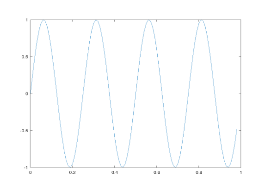
\includegraphics[width=6cm, height=4cm]{sineplot.png}
\end{figure}

\begin{lstlisting}[basicstyle=\small]

octave:4> y2 = cos(2*pi*4*t);
octave:5> plot(t,y1);
octave:6> hold on;
octave:7> plot(t, y2, 'r');
octave:8> xlabel('time')
octave:9> ylabel('value')
octave:10> legend('sin', 'cos')
octave:11> title('sine-cosine plot')
octave:12> print -dpng 'myPlot.png'
\end{lstlisting}

\begin{figure}[h]
  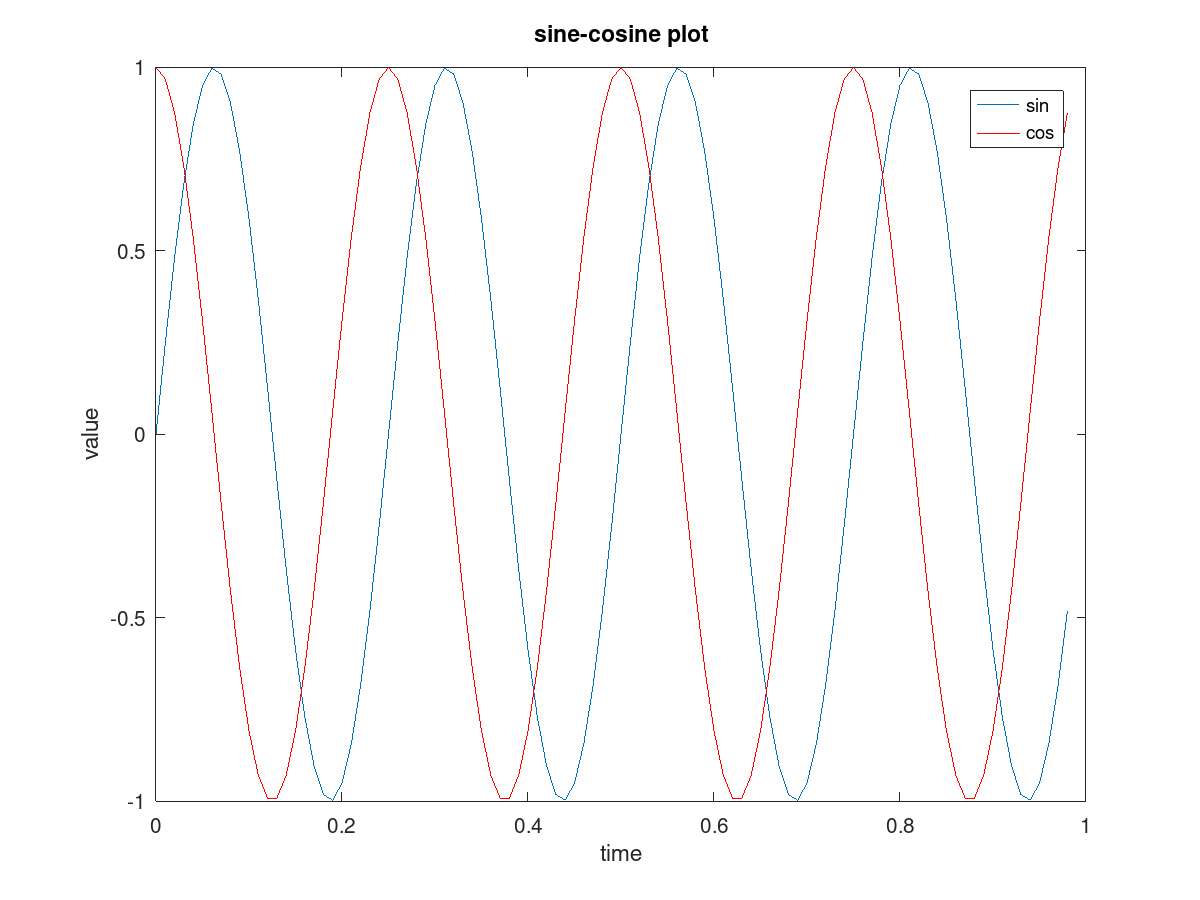
\includegraphics[width=6cm, height=4cm]{myPlot.png}
\end{figure}

\begin{lstlisting}[basicstyle=\small]

octave:13> close
octave:14> figure(1); plot(t, y1);
octave:15> figure(2); plot(t, y2);
octave:16> subplot(1,2,1);   % Divides plot a 1x2 grid
octave:17> plot(t,y1);
octave:18> subplot(1,2,2)
octave:19> plot(t,y2);
octave:20> axis([0.5 1 -1 1])
\end{lstlisting}

\begin{figure}[h]
  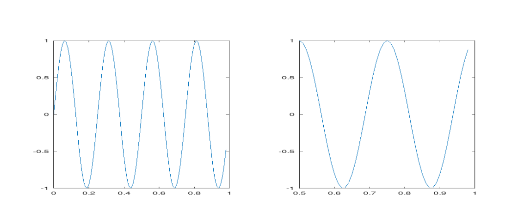
\includegraphics[width=12cm, height=4cm]{plot2.png}
\end{figure}

\vspace{5mm}
\subsubsection{Control Statements: for, while, if, else-if ...}

\begin{lstlisting}[basicstyle=\small]
octave:1> v = zeros(10,1)
v =

   0
   0
   0
   0
   0
   0
   0
   0
   0
   0

octave:2> for i=1:10,
> v(i) = 2^i;
> end;

octave:3> v
v =

      2
      4
      8
     16
     32
     64
    128
    256
    512
   1024

octave:4> i=1;
octave:5> while i <= 5,
> v(i) = 100;
> i = i+1;
> end;
octave:6> v
v =

    100
    100
    100
    100
    100
     64
    128
    256
    512
   1024

octave:7> i = 1;
octave:8> while true,
> v(i) = 999;
> i = i+1;
> if i == 6,
>   break;
> end;
> end;

octave:9> v
v =

    999
    999
    999
    999
    999
     64
    128
    256
    512
   1024

\end{lstlisting}


\end{document}

